% !TeX spellcheck = de_CH_frami
\section{Implementation}

\subsection{API}
\begin{frame}[fragile]
\frametitle{API}

\begin{itemize}
\item Die REST API besteht aus f�nf Endpunkten: /matches, /leagues, /courts, /users, /core
\item Beispiel: /leagues/join
\end{itemize}

\begin{lstlisting}
exports.join = function (req, res) {

    var league = req.league;
    var user = req.user;
    var userToPoints = new UserToPoints();
    userToPoints.user = req.user;
    userToPoints.save();

    league.users.push(userToPoints);
    user.leagues.push(league)

    console.log(league);
    league.save(function (err) {
        ....
\end{lstlisting}

\end{frame}

\subsection{Web Applikation}

\begin{frame}[fragile]
\frametitle{Web Applikation}

\begin{itemize}
\item JavaScript MVC Framework
\item JavaScript bezieht Models �ber API und stellt sie dar
\end{itemize}
\begin{lstlisting}
<section data-ng-controller="CourtsController" data-ng-init="find()">
    ....
        <table id="courtslist" class="table">
            <tr>
                <th>Name</th><th>Adresse</th><th>Verf�gbare Sportarten</th>
            </tr>

            <tr data-ng-repeat="court in courts" id="{{court._id}}" ng-click="go(court)"  onMouseover="this.bgColor='#DDDDDD'" onMouseout="this.bgColor='#FFFFFF'">
                <td data-ng-bind="court.name"></td>
                <td data-ng-bind="court.address"></td>
                <td data-ng-bind="court.sports"></td>
            </tr>
        </table>
....
\end{lstlisting}

\end{frame}
\subsection{Android Applikation}
\frame{\frametitle{Android Applikation}

\begin{itemize}
\item Stellt �ber die WebView die Mobil-Seite dar
\item Wurde generiert �ber GoNative.io
\end{itemize}


}
\subsection{Workflows}
\frame{\frametitle{Workflows}

\begin{itemize}
\item Komplexe Workflows
\item Einfaches Beispiel: automatische Herausforderung
\end{itemize}

	\begin{center}
	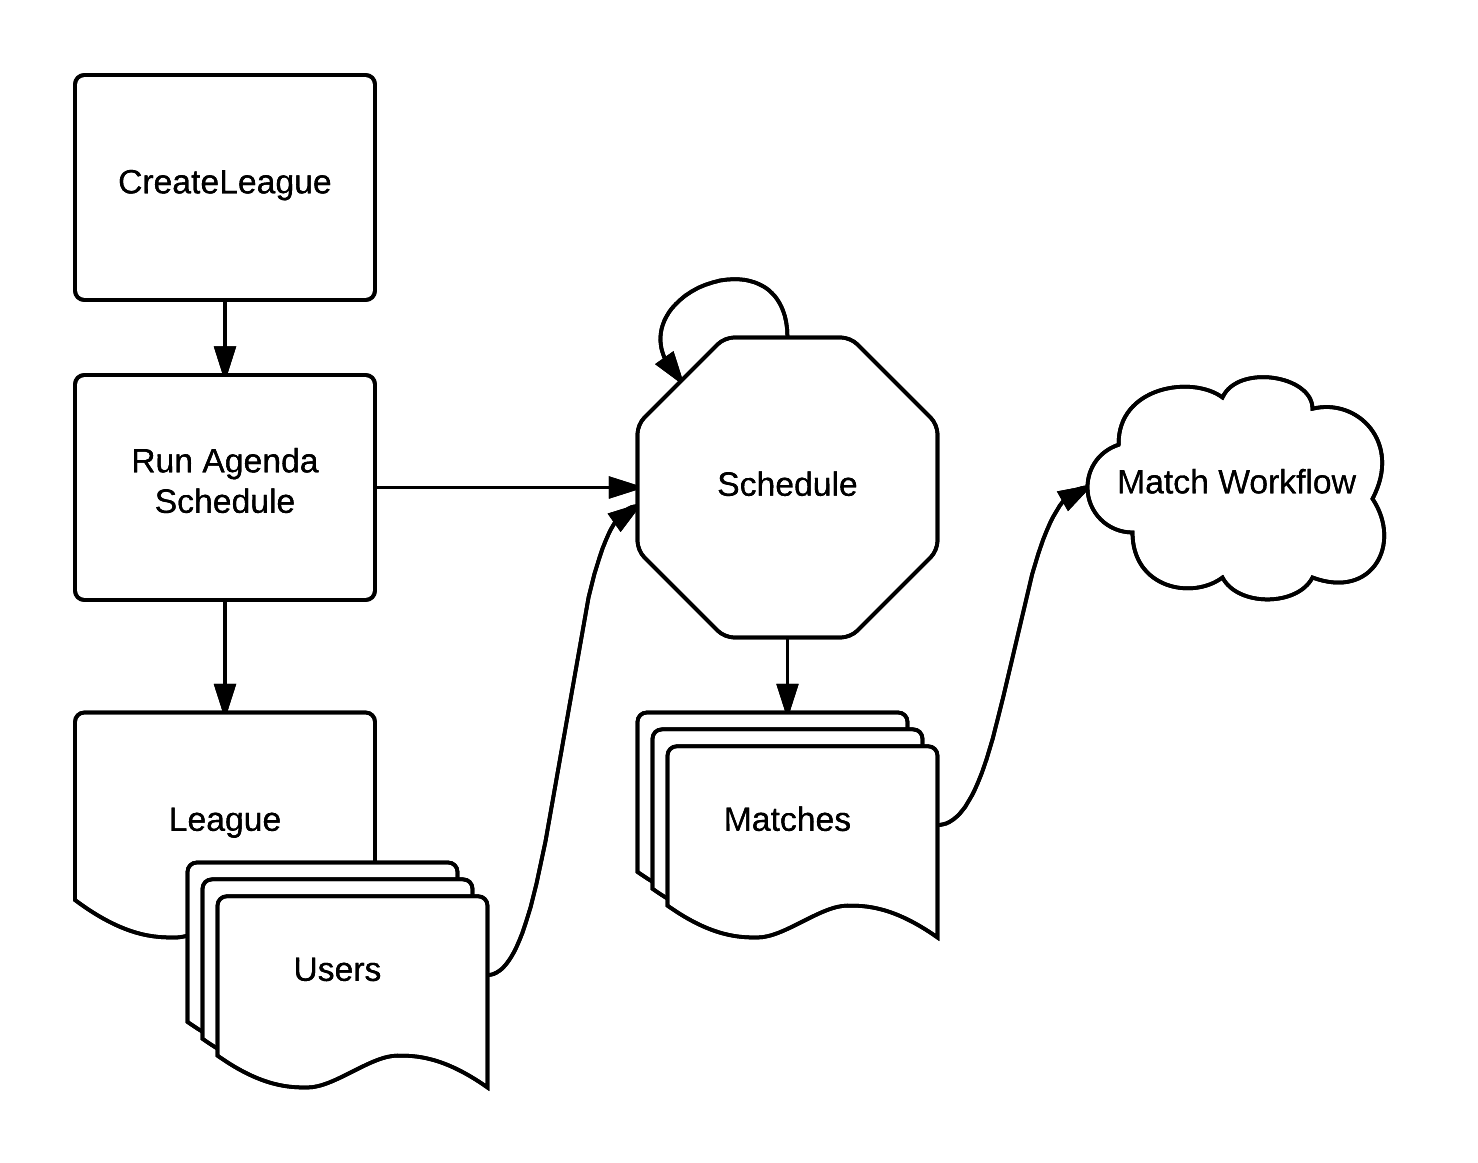
\includegraphics[scale=0.5]{pic/schedue_workflow.png}
	\end{center}

}